\documentclass[tikz, border=6pt]{standalone}
\IfFileExists{lmodern.sty}{\usepackage[T1]{fontenc}\usepackage{lmodern}}{}
\usepackage{amsmath,amssymb,bm}
\usepackage[scaled=0.95]{helvet}
\usetikzlibrary{arrows.meta}
\definecolor{Blue}{HTML}{3A76D8}
\definecolor{Orange}{HTML}{EE8133}
\definecolor{Ink}{HTML}{1F2937}
\tikzset{
  vertex/.style={/utils/exec={\colorlet{pytikzarg}{#1}}, circle, draw=pytikzarg!78!black, fill=pytikzarg!20, minimum size=7.5mm, inner sep=1pt, line width=0.7pt, font=\small},
  vertex/.default=Blue,
  graph edge/.style={Ink!65, line width=0.8pt},
  graph label/.style={font=\footnotesize, fill=white, inner sep=1.5pt},
}
\begin{document}
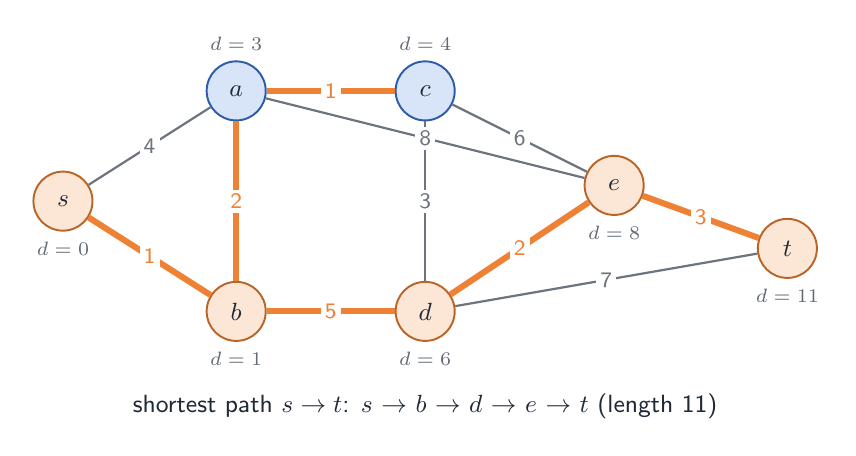
\begin{tikzpicture}[color=Ink, execute at begin picture={\sffamily}, line width=0.6pt, >={Stealth[length=5.5pt, width=4pt, inset=1.2pt]}, line join=round]
  % graph g: 7 nodes, 11 edges
  \node[vertex=Orange] (g-s) at (0,0) {$s$};
  \node[vertex=Blue] (g-a) at (2.2,1.4) {$a$};
  \node[vertex=Orange] (g-b) at (2.2,-1.4) {$b$};
  \node[vertex=Blue] (g-c) at (4.6,1.4) {$c$};
  \node[vertex=Orange] (g-d) at (4.6,-1.4) {$d$};
  \node[vertex=Orange] (g-e) at (7,0.2) {$e$};
  \node[vertex=Orange] (g-t) at (9.2,-0.6) {$t$};
  \draw[graph edge] (g-s) -- node[graph label] {4} (g-a);
  \draw[graph edge, Orange, line width=2.2pt] (g-s) -- node[graph label, text=Orange] {1} (g-b);
  \draw[graph edge, Orange, line width=2.2pt] (g-b) -- node[graph label, text=Orange] {2} (g-a);
  \draw[graph edge, Orange, line width=2.2pt] (g-a) -- node[graph label, text=Orange] {1} (g-c);
  \draw[graph edge, Orange, line width=2.2pt] (g-b) -- node[graph label, text=Orange] {5} (g-d);
  \draw[graph edge] (g-c) -- node[graph label] {3} (g-d);
  \draw[graph edge] (g-c) -- node[graph label] {6} (g-e);
  \draw[graph edge, Orange, line width=2.2pt] (g-d) -- node[graph label, text=Orange] {2} (g-e);
  \draw[graph edge] (g-d) -- node[graph label] {7} (g-t);
  \draw[graph edge, Orange, line width=2.2pt] (g-e) -- node[graph label, text=Orange] {3} (g-t);
  \draw[graph edge] (g-a) -- node[graph label] {8} (g-e);
  \node[anchor=north, font=\scriptsize, text=Ink!70] at (g-s.south) {$d=0$};
  \node[anchor=south, font=\scriptsize, text=Ink!70] at (g-a.north) {$d=3$};
  \node[anchor=north, font=\scriptsize, text=Ink!70] at (g-b.south) {$d=1$};
  \node[anchor=north, font=\scriptsize, text=Ink!70] at (g-d.south) {$d=6$};
  \node[anchor=south, font=\scriptsize, text=Ink!70] at (g-c.north) {$d=4$};
  \node[anchor=north, font=\scriptsize, text=Ink!70] at (g-e.south) {$d=8$};
  \node[anchor=north, font=\scriptsize, text=Ink!70] at (g-t.south) {$d=11$};
  \node[font=\small] at (4.6,-2.6) {shortest path $s \to t$: $s$ $\to$ $b$ $\to$ $d$ $\to$ $e$ $\to$ $t$ (length 11)};
\end{tikzpicture}
\end{document}
